\part{Memory Management in C}\toc
\begin{frame}{Memory Management in C}
  \begin{block}{Introduction}
    \begin{itemize}
    \item Main specificity of the C language: \alert{\textbf{Memory Management}}
    \item You have \textbf{full control} over the memory in C
    \item That gives you the full power \ldots\ to shoot you in the foot
    \end{itemize}
  \end{block}

  \begin{block}{Lecture agenda}
    \begin{itemize}
    \item First explore the basic notions over memory
      \begin{itemize}
      \item Local and Global variables; Scope and Lifetime; Notion of Address
        and Pointers
      \end{itemize}

    \item Then, (quick) look at the system side of memory management
      \begin{itemize}
      \item Memory Layout of a typical UNIX Process (more details in RS next year)
      \end{itemize}

    \item Finally, go into the full details of memory allocation/deallocation
      \begin{itemize}
      \item Student's hated malloc and associated madness
      \end{itemize}
    \end{itemize}
  \end{block}
\end{frame}
%%%%%%%%%%%%%%%%%%%%%%%%%%%%%%%%%%%%%%%%%%%%%%%%%%%%%%%%%%%%%%%%%%%%%%%%%%%%%%%%%%%%%%%%%%%%%%%%%
\section{Static Memory}
\subsection{Variables in C}
\begin{Coupe}
\begin{frame}{Variables in C}
  \begin{block}{Kind of identifiers in C}
    \begin{itemize}
    \item Little difference between variables and functions: they are all
      \textbf{\alert{identifiers}}
    \item Every C identifiers can be either \textbf{\alert{global}} or \textbf{\alert{local}}
    \item Main differences: \textbf{\alert{scope}}
      (visibility) and \textbf{\alert{lifetime}}
    \end{itemize}
  \end{block}\vspace{-.5\baselineskip}

  \begin{block}{Local Identifiers}
    \begin{itemize}
    \item They are declared within a function
    \item \structure{Side note:} nested functions are forbidden in standard C\\
      {\small \texttt{gcc} allows nested functions as a language extension -- I
        recommend not using them}
    \item \structure{\textbf{Scope:}} Usable from the block where they are declared
    \item \structure{\textbf{Lifetime:}} Valid only until the execution leaves
      the block
    \end{itemize}
  \end{block}\vspace{-.5\baselineskip}

  \begin{block}{Global identifiers}
    \begin{itemize}
    \item They are declared outside of any function 
    \item \structure{\textbf{Scope:}} Usable from the whole project
    \item \structure{\textbf{Lifetime:}}  permanent
    \item (yes, there is no such thing in Java)
    \end{itemize}
  \end{block}
\end{frame}
%%%%%%%%%%%%%%%%%%%%%%%%%%%%%%%%%%%%%%%%%%%%%%%%%%%%%%%%%%%%%%%%%%%%%%%%%%%%%%%%%%%%%%%%%%%%%%%%%
\begin{frame}{First Weird Code with Variables}
  \vspace{-.5\baselineskip}
  \framebox{\resizebox{.45\linewidth}{!}{
  \begin{minipage}{.3\linewidth}
\tt  \begin{tabbing}
\alert<2| handout:0>{~1:int a;}\\
~2:int main() \{\\
\alert<3| handout:0>{~3:~~int b;}\\
\alert<4| handout:0>{~3:~~a=0;}\\
\alert<5| handout:0>{~4:~~b=a;}\\
\alert<6| handout:0>{~5:~~printf("a:~\%d, b:~\%d$\backslash$n",a,b);}\\
\alert<7| handout:0>{~6:~~a += 5;}\\
~7:~~\{\\
\alert<8| handout:0>{~8:~~~~int a;}\\
\alert<9| handout:0>{~9:~~~~printf("a:~\%d, b:~\%d$\backslash$n",a,b);}\\
10:~~\}\\
\alert<10| handout:0>{11:~~a += 5;}\\
12:~~\{\\
\alert<11| handout:0>{13:~~~~int b=a;}\\
\alert<12| handout:0>{14:~~~~printf("a:~\%d, b:~\%d$\backslash$n",a,b);}\\
\alert<13| handout:0>{15:~~~~b += 5;}\\
16:~~~~\{\\
\alert<14|handout:0>{17:~~~~~~int b=0;}\\
\alert<15| handout:0>{18:~~~~~~printf("a:~\%d, b:~\%d$\backslash$n", a,b);}\\
19:~~~~\}\\
\alert<16| handout:0>{20:~~~~printf("a:~\%d, b:~\%d$\backslash$n", a,b);}\\
21:~~\}\\
\alert<17| handout:0>{22:~~printf("a:~\%d, b:~\%d$\backslash$n",a,b);}\\
23:~~return 0;\\
24:\}  
  \end{tabbing}          
  \end{minipage}}}\hfill%
  \begin{minipage}{.5\linewidth}
    \begin{block}{Remarks}
      \begin{itemize}
      \item Yes, we can use anonymous blocks
      \item We can declare variables in there
      \item We can override variables this way
      \item All this is possible in Java too!
      \end{itemize}
    \end{block}\vspace{-\baselineskip}

    \begin{block}{What does this code do?}\medskip
      \begin{minipage}{.5\linewidth}
        \begin{itemize}
        \item<2->[l1] $a$\visible<8->{$_1$} \framebox{\visible<4->{0}}
        \item<3->[l3] $b$\visible<8->{$_3$} \framebox{\visible<5->{0}}
        \item<6->[l5] \texttt{a:~0; b:~0}
        \item<7->[l6] $a$\visible<8->{$_1$} \framebox{5}
        \item<8->[l8] $a_8$ \framebox{??}
        \item<9->[l9] \texttt{a:~??;~b:~0}
        \item<10->[l11] $a_1$ \framebox{10}
        \end{itemize}        
      \end{minipage}%
      \begin{minipage}{.5\linewidth}
        \begin{itemize}
        \item<11->[l13] $b_{13}$ \framebox{10}
        \item<12->[l14] \texttt{a:~10;~b:~10}
        \item<13->[l15] $b_{13}$ \framebox{15}
        \item<14->[l17] $b_{17}$ \framebox{0}
        \item<15->[l18] \texttt{a:~10;~b:~0}
        \item<16->[l20] \texttt{a:~10;~b:~15}
        \item<17->[l22] \texttt{a:~10;~b:~0}
        \end{itemize}
      \end{minipage}
    \end{block}\vspace{-.4\baselineskip}
    \begin{alertblock}<18->{Ok, but how to \textbf{understand} it?}
      \begin{itemize}\vspace{-\baselineskip}
      \item<19-> Think of a stack containing locals
      \end{itemize}
    \end{alertblock}
  \end{minipage}
\end{frame}
%%%%%%%%%%%%%%%%%%%%%%%%%%%%%%%%%%%%%%%%%%%%%%%%%%%%%%%%%%%%%%%%%%%%%%
\begin{frame}{Variables are Stored on a Stack}
  \vspace{-.5\baselineskip}
  \framebox{\resizebox{.45\linewidth}{!}{
  \begin{minipage}{.3\linewidth}
\tt  \begin{tabbing}
\alert<2| handout:0>{~1:int a;}\\
~2:int main() \{\\
\alert<3| handout:0>{~3:~~int b;}\\
\alert<4| handout:0>{~3:~~a=0;}\\
\alert<5| handout:0>{~4:~~b=a;}\\
\alert<6| handout:0>{~5:~~printf("a:~\%d, b:~\%d$\backslash$n",a,b);}\\
\alert<7| handout:0>{~6:~~a += 5;}\\
~7:~~\{\\
\alert<8| handout:0>{~8:~~~~int a;}\\
\alert<9| handout:0>{~9:~~~~printf("a:~\%d, b:~\%d$\backslash$n",a,b);}\\
10:~~\}\\
\alert<10| handout:0>{11:~~a += 5;}\\
12:~~\{\\
\alert<11| handout:0>{13:~~~~int b=a;}\\
\alert<12| handout:0>{14:~~~~printf("a:~\%d, b:~\%d$\backslash$n",a,b);}\\
\alert<13| handout:0>{15:~~~~b += 5;}\\
16:~~~~\{\\
\alert<14|handout:0>{17:~~~~~~int b=0;}\\
\alert<15| handout:0>{18:~~~~~~printf("a:~\%d, b:~\%d$\backslash$n", a,b);}\\
19:~~~~\}\\
\alert<16| handout:0>{20:~~~~printf("a:~\%d, b:~\%d$\backslash$n", a,b);}\\
21:~~\}\\
\alert<17| handout:0>{22:~~printf("a:~\%d, b:~\%d$\backslash$n",a,b);}\\
23:~~return 0;\\
24:\}  
  \end{tabbing}          
  \end{minipage}}}\hfill%
  \begin{minipage}{.5\linewidth}
    \begin{block}{Explaining the outputs}\medskip
      \begin{minipage}{.5\linewidth}
        \begin{itemize}
          \alert<6|handout:0>{\item[l5] \texttt{a:~0; b:~0}}
          \alert<9|handout:0>{\item[l9] \texttt{a:~??;~b:~0}}
          \alert<12|handout:0>{\item[l14] \texttt{a:~10;~b:~10}}
        \end{itemize}      
      \end{minipage}\begin{minipage}{.5\linewidth}
        \begin{itemize}
          \alert<15|handout:0>{\item[l18] \texttt{a:~10;~b:~0}}
          \alert<16|handout:0>{\item[l20] \texttt{a:~10;~b:~15}}
          \alert<17|handout:0>{\item[l22] \texttt{a:~10;~b:~0}}
        \end{itemize}
      \end{minipage}
    \end{block}
    \begin{block}{The stack over time}
      \begin{itemize}
      \item Higher variables mask deeper ones
      \end{itemize}
    \end{block}
    \begin{minipage}[b]{.18\linewidth} %% l5
      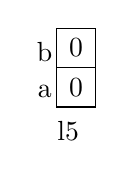
\begin{tikzpicture}
        \visible<2->{
          \draw (0.35, 0.2) node {a};
          \draw (0.5,0) rectangle (1,.5);            
        }
        \draw<4-> (.75,.25) node {0}; 
        \visible<3->{
          \draw (0.35, 0.7) node {b};
          \draw (.5,0.5) rectangle (1,1);
        }
        \draw<5-> (.75,.75) node {0};
        \visible<6->{
          \draw (.65,-.3) node {\structure{l5}};
        }
      \end{tikzpicture}        
    \end{minipage}$\!\!$\begin{minipage}[b]{.18\linewidth} %% l9
      \visible<7->{
        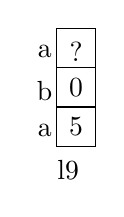
\begin{tikzpicture}
          \draw (0.35, 0.2) node {a};
          \draw (0.5,0) rectangle (1,.5);
          \draw (.75,.25) node {5};
          
          \draw (0.35, 0.7) node {b};
          \draw (.5,0.5) rectangle (1,1);
          
          \draw<5-> (.75,.75) node {0};
          
          \visible<8->{
            \draw (0.35, 1.2) node {a};
            \draw (.5,1) rectangle (1,1.5);
            \draw (.75, 1.2) node {?};
          }
          \visible<9->{
            \draw (.65,-.3) node {\structure{l9}};
          }
        \end{tikzpicture}
      }
    \end{minipage}$\!\!$\begin{minipage}[b]{.18\linewidth} %% l14
      \visible<10->{
        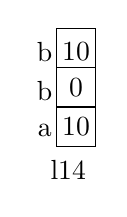
\begin{tikzpicture}
          \draw (0.35, 0.2) node {a};
          \draw (0.5,0) rectangle (1,.5);
          \draw (.75,.25) node {10};
          
          \draw (0.35, 0.7) node {b};
          \draw (.5,0.5) rectangle (1,1);
          \draw (.75,.75) node {0};
          
          \visible<11->{
            \draw (0.35, 1.2) node {b};
            \draw (.5,1) rectangle (1,1.5);
            \draw<11-> (.75, 1.2) node {10};
          }
          \visible<12->{
            \draw (.65,-.3) node {\structure{l14}};
          }          
        \end{tikzpicture}
      }
    \end{minipage}$\!\!$\begin{minipage}[b]{.18\linewidth} %% l18
      \visible<13->{
        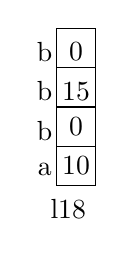
\begin{tikzpicture}
          \draw (0.35, 0.2) node {a};
            \draw (0.5,0) rectangle (1,.5);
            \draw (.75,.25) node {10};
            
            \draw (0.35, 0.7) node {b};
            \draw (.5,0.5) rectangle (1,1);
            \draw (.75,.75) node {0};

            \draw (0.35, 1.2) node {b};
            \draw (.5,1) rectangle (1,1.5);
            \draw (.75, 1.2) node {15};

            \visible<14->{
              \draw (0.35, 1.7) node {b};
              \draw (.5,1.5) rectangle (1,2);
              \draw (.75, 1.7) node {0};
            }
            \visible<15->{
              \draw (.65,-.3) node {\structure{l18}};
            }
          \end{tikzpicture}
        }
    \end{minipage}$\!\!$\begin{minipage}[b]{.18\linewidth} %% l20
        \visible<16->{
          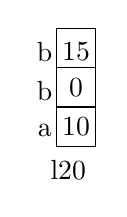
\begin{tikzpicture}
            \draw (0.35, 0.2) node {a};
            \draw (0.5,0) rectangle (1,.5);
            \draw (.75,.25) node {10};
            
            \draw (0.35, 0.7) node {b};
            \draw (.5,0.5) rectangle (1,1);
            \draw (.75,.75) node {0};
            
            \draw (0.35, 1.2) node {b};
            \draw (.5,1) rectangle (1,1.5);
            \draw (.75, 1.2) node {15};
            
            \draw (.65,-.3) node {\structure{l20}};
          \end{tikzpicture}            
        }
    \end{minipage}$\!\!$\begin{minipage}[b]{.18\linewidth} %% l22
        \visible<17->{
          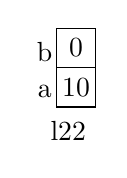
\begin{tikzpicture}
            \draw (0.35, 0.2) node {a};
            \draw (0.5,0) rectangle (1,.5);
            \draw (.75,.25) node {10};
            
            \draw (0.35, 0.7) node {b};
            \draw (.5,0.5) rectangle (1,1);
            \draw (.75,.75) node {0};
            
            \draw (.65,-.3) node {\structure{l22}};
          \end{tikzpicture}            
        }
    \end{minipage}
      
  \end{minipage}
\end{frame}
%%%%%%%%%%%%%%%%%%%%%%%%%%%%%%%%%%%%%%%%%%%%%%%%%%%%%%%%%%%%%%%%%%%%%%%%
\begin{frame}{Function Parameters}  
  \begin{block}{Parameters are stacked too}
    \begin{itemize}
    \item One \textbf{\alert{stack frame}} per function (containing local vars and parameters)
    \item Stack frame: created on function call,  destructed when the function returns
    \item Parameters can be seen as local variables (can even be modified)
    \item Parameters are \textbf{\alert{passed by value}} (ie, copied over)
    \end{itemize}
  \end{block}  

  \begin{columns}
    \begin{column}{.5\linewidth}
      \framebox{\begin{minipage}{.3\linewidth}
          \tt\footnotesize  \begin{tabbing}
            \alert<3|handout:0>{int \textbf{max}(int a, int b) \{}\\
            \alert<4|handout:0>{~~return a$>$b ? a : b;}\\
            \}\\
            \\
            \alert<1|handout:0>{int \textbf{main}() \{}\\
            \alert<1|handout:0>{~~int x=12;}\\
            \alert<1|handout:0>{~~int y=42;}\\
            \alert<5|handout:0>{~~return \alert<2|handout:0>{max(x,y);}}\\
            \}
          \end{tabbing}
        \end{minipage}}    
    \end{column}
    \begin{column}{.3\linewidth}
      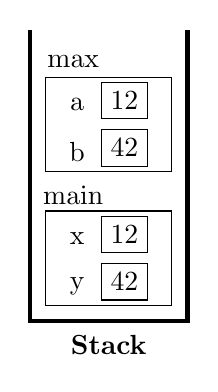
\begin{tikzpicture}
        % Stack container
        \draw[ultra thick] (0,3.7) -- (0,0) -- (2,0) -- (2, 3.7);
        \node at (1,-.3) {\bf Stack};
        
        % Stack frame of main 
        \draw (.2,.2) rectangle (1.8,1.4);
        
        \node at (1.2,.5) [shape=rectangle,draw]  {42} ;
        \node at (.6,.45) {y};
        
        \node at (1.2,1.1) [shape=rectangle,draw]  {12} ;
        \node at (.6,1.05) {x};
        
        \node at (.55,1.6) {main};
        
        \visible<3-4>{
          % Stack frame of max
          \draw (.2,1.9) rectangle (1.8,3.1);
          
          \node at (1.2,2.2) [shape=rectangle,draw]  {42} ;
          \node at (.6,2.15) {b};
          
          \node at (1.2,2.8) [shape=rectangle,draw]  {12} ;
          \node at (.6,2.75) {a};
          
          \node at (.55,3.3) {max};
        }
      \end{tikzpicture}
    \end{column}
  \end{columns}
\end{frame}
%%%%%%%%%%%%%%%%%%%%%%%%%%%%%%%%%%%%%%%%%%%%%%%%%%%%%%%%%%%%%%%%%%%%%%%%
\begin{frame}{Function Parameters Tricks}  
  \begin{block}{Parameters are passed by value}
    \begin{itemize}
    \item We just said that but it is not as natural as it seems
    \item It forbids any side effects on parameters
    \item<7> There is no way to avoid passing by value
    \item<7> But pointers help: scanf manages to ``modify its arguments''
    \end{itemize}
  \end{block}  

  \begin{columns}
    \begin{column}{.35\linewidth}
      \framebox{\begin{minipage}{.3\linewidth}
          \tt\footnotesize  \begin{tabbing}
            \alert<3|handout:0>{void \textbf{triple}(int a) \{}\\
            \alert<4|handout:0>{~~a=a*3;}\\
            \alert<5|handout:0>{~~return;}\\
            \}\\
            \\
            \alert<1|handout:0>{int \textbf{main}() \{}\\
            \alert<1|handout:0>{~~int x=12;}\\
            \alert<2|handout:0>{~~triple(x);}\\
            \alert<6|handout:0>{~~printf("x:~\%d",x);}\\
            \alert<7|handout:0>{~~return EXIT\_SUCCESS;}\\
            \}
          \end{tabbing}
        \end{minipage}}    
    \end{column}
    \begin{column}{.25\linewidth}
      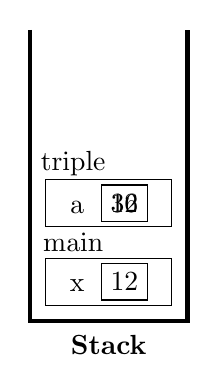
\begin{tikzpicture}
        % Stack container
        \draw[ultra thick] (0,3.7) -- (0,0) -- (2,0) -- (2, 3.7);
        \node at (1,-.3) {\bf Stack};
        
        % Stack frame of main 
        \visible<1-6>{
          \draw (.2,.2) rectangle (1.8,.8);
          
          \node at (1.2,.5) [shape=rectangle,draw]  {12} ;
          \node at (.6,.45) {x};
                
          \node at (.55,1) {main};
        }

        \visible<3-4>{
          % Stack frame of max
          \draw (.2,1.2) rectangle (1.8,1.8);
          
          \node<3|handout:0> at (1.2,1.5) [shape=rectangle,draw]  {12} ;
          \node<4> at (1.2,1.5) [shape=rectangle,draw]  {36} ;
          \node at (.6,1.45) {a};
          
          \node at (.55,2) {triple};
        }
      \end{tikzpicture}
    \end{column}
    \begin{column}{.3\linewidth}
      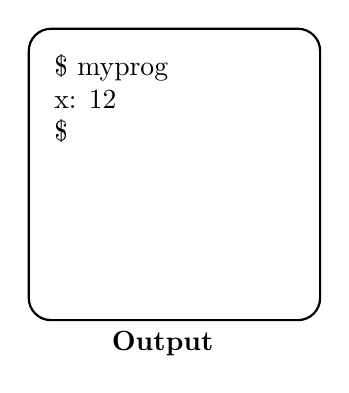
\begin{tikzpicture}
        \draw[thick,rounded corners=8pt] (0,0) rectangle (3.7,3.7);
        \node at (1.7,-.3) {\bf Output};

        \node[right] at (.2,3.2) {\$ myprog};
        \node<6->[right] at (.2,2.8) {x: 12};
        \node<7->[right] at (.2,2.4) {\$};

      \end{tikzpicture}
    \end{column}
  \end{columns}
\end{frame}
%%%%%%%%%%%%%%%%%%%%%%%%%%%%%%%%%%%%%%%%%%%%%%%%%%%
\begin{frame}{Weird Code with Function Calls}
  \vspace{-.5\baselineskip}
  \framebox{\resizebox{.4\linewidth}{!}{
  \begin{minipage}{.3\linewidth}
\footnotesize\tt  \begin{tabbing}
~1:int a;\\
~2:int main() \{\\
~3:~~int b;\\
~3:~~a=0;\\
~4:~~b=a;\\
~5:~~printab(a,b);\\
~6:~~a += 5;\\
~7:~~\{~int a;\\
~8:~~~~printab(a,b);\\
~9:~~\}\\
10:~~a += 5;\\
11:~~\{~int b=a;\\
12:~~~~printab(a,b);\\
13:~~~~b += 5;\\
14:~~~~\{~int b=0;\\
15:~~~~~~printab(a,b);\\
16:~~~~\}\\
17:~~~~printab(a,b);\\
18:~~\}\\
19:~~printab(a,b);\\
20:~~return 0;\\
21:\}\\
22:int printab(\alert<3>{int \only<1-2>{b}\only<3>{\framebox{b}}, int \only<1-2>{a}\only<3>{\framebox{a}}}) \{\\
23:~~printf("a:\%d, b:\%d$\backslash$n",a,b);~~~\\
24:\}
  \end{tabbing}          
  \end{minipage}}}\hfill%
  \begin{minipage}{.56\linewidth}
    \begin{block}{Code similar to previously}
      \begin{itemize}
      \item Call printab() for display, not printf()
      \end{itemize}
    \end{block}
    \begin{block}<2->{Old Output}\medskip
      \begin{minipage}{.5\linewidth}
        \begin{itemize}
          \item[l5] \texttt{a:~0; b:~0}
          \item[l9] \texttt{a:~??;~b:~0}
          \item[l14] \texttt{a:~10;~b:~10}
        \end{itemize}      
      \end{minipage}\begin{minipage}{.5\linewidth}
        \begin{itemize}
          \item[l18] \texttt{a:~10;~b:~0}
          \item[l20] \texttt{a:~10;~b:~15}
          \item[l22] \texttt{a:~10;~b:~0}
        \end{itemize}
      \end{minipage}      
    \end{block}

    \begin{block}<2->{New Output}\medskip
      \begin{minipage}{.5\linewidth}
        \begin{itemize}
          \item[l5] \texttt{a:0; b:0}
          \item[l9] \texttt{a:0;~b:??}
          \item[l14] \texttt{a:10;~b:10}
        \end{itemize}      
      \end{minipage}\begin{minipage}{.5\linewidth}
        \begin{itemize}
          \item[l18] \texttt{a:0;~b:10}
          \item[l20] \texttt{a:15;~b:10}
          \item[l22] \texttt{a:0;~b:10}
        \end{itemize}
      \end{minipage}      
    \end{block}
    
    \medskip\visible<2->{\concept{This is all inverted!}}

    \begin{block}<2->{The trick comes from\ldots}
      \begin{itemize}
      \item<3> printab's parameters, which are inverted
      \end{itemize}      
    \end{block}
  \end{minipage}
\end{frame}
%%%%%%%%%%%%%%%%%%%%%%%%%%%%%%%%%%%%%%%%%%%%%%%%%%%%%%%%%%%
\begin{frame}{The keyword static}
  \concept{This little keyword has two (quite differing) meanings}

  \begin{block}{When applied to global identifiers}
    \begin{itemize}
    \item \structure{Reduces visibility:} from ``the whole project'' to ``this
      file'' {\small (as if it were local)}
    \item \structure{Lifetime} remains unchanged

    \item \structure{Java equivalent:} private
    \end{itemize}
  \end{block}

  \begin{block}{When applied to local identifiers}
    \begin{itemize}
    \item \structure{Increases lifetime:} from ``for this call'' to ``for ever''
      {\small (as if it were global)}
    \item \structure{Visibility} remains unchanged
    \item \structure{Similar concept in Java:} static
    \end{itemize}
  \end{block}

  \visible<2->{
  \begin{center}
    \begin{tabular}{|l|c|c|}\cline{2-3}
      \multicolumn{1}{c|}{}      &\structure{Visibility}&\structure{Lifetime}\\\hline
      \structure{Functions}      &Whole Project&For Ever\\\hline
      \structure{Global Variable}&Whole Project&For Ever\\\hline
      \visible<3->{\structure{Static Global Variable}&This File Only&For Ever}\\\hline%visible<3->{\hline}
      \visible<3->{\structure{Static Local Variable}&Current Block&For Ever}\\\hline
      \structure{Local Variable}&Current Block&Until End of Block\\\hline      
    \end{tabular}    
  \end{center}}
\end{frame}
%%%%%%%%%%%%%%%%%%%%%%%%%%%%%%%%%%%%%%%%%%%%%%%%%%%%%%%%%%%%%%%%%%%%%%%%%
\begin{frame}{More on Static Local Variables}
  \begin{columns}
    \begin{column}{.35\linewidth}
      \framebox{\begin{minipage}{.45\linewidth}
          \tt\footnotesize  \begin{tabbing}
            \alert<3,8|handout:0>{int \textbf{nextInt}() \{}\\
            \alert<3|handout:0>{~~\alert<8|handout:0>{\textbf{\textrm{static}} int res}=0;}\\
            \alert<4,9|handout:0>{~~res+=1;}\\
            \alert<5,10|handout:0>{~~return res;}\\
            \}\\
            \\
            \alert<1|handout:0>{int \textbf{main}() \{}\\
            \alert<6|handout:0>{~~printf("next:\%d",\alert<2|handout:0>{nextInt()});}\\
            \alert<11|handout:0>{~~printf("next:\%d",\alert<7|handout:0>{nextInt()});}\\
            \alert<12|handout:0>{~~return EXIT\_SUCCESS;}\\
            \}
          \end{tabbing}
        \end{minipage}}    
    \end{column}
    \begin{column}{.15\linewidth}
      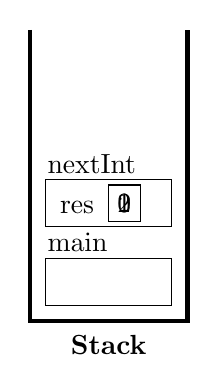
\begin{tikzpicture}
        % Stack container
        \draw[ultra thick] (0,3.7) -- (0,0) -- (2,0) -- (2, 3.7);
        \node at (1,-.3) {\bf Stack};
        
        % Stack frame of main 
        \visible<1-11>{
          \draw (.2,.2) rectangle (1.8,.8);
          \node[right] at (.1,1) {main};
        }

        \visible<3-5,8-9>{
          % Stack frame of nextInt
          \draw (.2,1.2) rectangle (1.8,1.8);
          
          \node<3|handout:0> at (1.2,1.5) [shape=rectangle,draw]  {0} ;
          \node<4-5,8|handout:0> at (1.2,1.5) [shape=rectangle,draw]  {1} ;
          \node<9-10> at (1.2,1.5) [shape=rectangle,draw]  {2} ;
          \node at (.6,1.45) {res};
          
          \node[right] at (.1,2) {nextInt};
        }
      \end{tikzpicture}
    \end{column}
    \begin{column}{.24\linewidth} 
      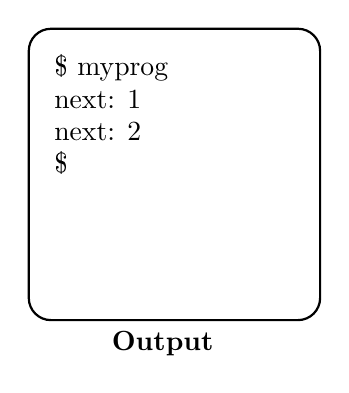
\begin{tikzpicture}
        \draw[thick,rounded corners=8pt] (0,0) rectangle (3.7,3.7);
        \node at (1.7,-.3) {\bf Output};

        \node[right] at (.2,3.2) {\$ myprog};
        \node<6->[right] at (.2,2.8) {next: 1};
        \node<11->[right] at (.2,2.4) {next: 2};
        \node<12->[right] at (.2,2) {\$};

      \end{tikzpicture}
    \end{column}
  \end{columns}

  \begin{itemize}
  \item<8-> The value remains from one call to another (initializer evaluated only once)
  \item<12-> This variable cannot live on the stack: would have been erased by
    another call
  \item<12-> Understanding where it lives require some more background on the
    system\\
    {(actually, the globals are not on the stack either)}
  \end{itemize}
\end{frame}
%%%%%%%%%%%%%%%%%%%%%%%%%%%%%%%%%%%%%%%%%%%%%%%%%%%%%%%%%%%%%%%%%%%%%%%%%%%%%%%%%%%%
\subsection{Processes Memory Layout}
\begin{frame}{Processes Memory Layout}
  \begin{block}{Primer from Next Year in System Course}
    \begin{itemize}
    \item The memory of each process is split in 3 big \textbf{\alert{segments}}
    \item Heap is for the manually managed memory (see in half an hour)
    \item<2-> If more stack frames needed, the size of the stack grows toward
      the heap\\
      Conversely, the heap can grow toward the stack
    \item<3-> Between Heap and Stack, there is a hole \visible<4->{in the
        addressing space}
    \item<3-> If that hole becomes full (stack reaches heap), the process runs out of memory
    \item This is a simplification, but the ideas are there
    \end{itemize}

    \begin{center}
    \begin{tikzpicture}
      \draw (0,0) -- (6,0) -- (6,1) -- (0,1) -- (0,0);
      \draw (7.8,0) -- (10.3,0) -- (10.3,1) -- (7.8,1) -- (7.8,0);
      \draw (3,0) -- (3,1);
      \node at (1.5,0.73) {\textbf{Data}};
      \node at (1.5,0.25) {Code+Globals};

      \node at (4.5,0.73) {\textbf{Heap}};
      \node at (4.5,0.25) {Dynamic Memory};

      \node at (9,0.73) {\textbf{Stack}};
      \node at (9,0.25) {Stack Frames};
      \visible<2->{
        \draw[-stealth',thick] (6,.5) -- (6.5,.5);
        \draw[-stealth',thick] (7.8,.5) -- (7.3,.5);
      }
      
      \node<3-> at (6.9,.5) {$\emptyset$};
      \visible<4->{        
        \node at (0,-.2) {0};
        \node at (10.3,-.2) {4Gb};
      }
    \end{tikzpicture}
    \end{center}
  \end{block}\vspace{-1.5\baselineskip}

  \begin{block}<5->{Where do symbols live?}\medskip
    \begin{minipage}{.4\linewidth}
      \begin{itemize}
      \item \structure{Functions:} in Data segment
      \item \structure{Globals:} in Data segment\\
        ~
      \end{itemize}      
    \end{minipage}~%
    \begin{minipage}{.6\linewidth}
      \begin{itemize}
      \item \structure{Locals:} in Stack segment
      \item \structure{Static Locals:} in Data segment\\
        {\small(just like globals!)}
      \end{itemize}      
    \end{minipage}~
  \end{block}
\end{frame}
%%%%%%%%%%%%%%%%%%%%%%%%%%%%%%%%%%%%%%%%%%%%%%%%%%%%%%%%%%%%%%%%%%%%%
\subsection{Addresses}
\begin{frame}{More on Memory}
  \begin{block}{Solving the Enigma of Static Locals Storage raises New Questions}
    \begin{itemize}
    \item What is the addressing space?
      \visible<2->{\structure{$\leadsto$ This is another name for ``memory''}}
    \item How to get a valid mental representation of the memory?\\
      \visible<3->{\structure{$\leadsto$ Think of a very large array of
          cells. Each cell is 1 byte (8 bits) wide.}
      \begin{center}
        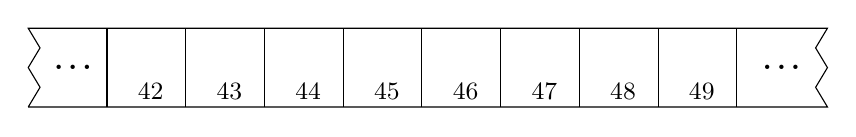
\begin{tikzpicture}
          \draw(0,0) -- (10.15,0) -- (10,.25) -- (10.15,.5) -- (10,.75) --
               (10.15,1) -- (0,1) -- (.15,.75) -- (0,.5) -- (.15,.25) -- (0,0);
          \foreach \i in { 1,2,3,4,5,6,7,8,9 } {
            \draw(\i,0) -- (\i,1);
          }
          \node at (.6,.5) {\textbf{\ldots}};
          \node at (9.6,.5) {\textbf{\ldots}};
          \visible<4->{
            \foreach \i in { 1,2,3,4,5,6,7,8 } {
              \node at (\i+.5,0.2) {\small \pgfmathtruncatemacro{\res}{41pt+\i} \res};;
            }
          }
        \end{tikzpicture}        
      \end{center}}
    \item What is an address?
      \visible<4->{\structure{$\leadsto$ Memory cells are numbered.\\ 
          The \textbf{\alert{address}} of a given memory cell is its number in rank}}
    \item Why the stack bottom at 4Gb? \visible<5->{\structure{$\leadsto$
          Because this is MAXINT on 32bits\\
          And the picture supposed that we were in 32bits for simplicity sake. }}
    \item Where is my stack if my laptop does not have 4Gb?
      \begin{itemize}
      \item<6-> \structure{Within the process, we are speaking of \textit{virtual
          addresses}}
      \item<6-> \structure{They get converted into \textit{physical ones} by the OS}
      \item<6-> \structure{But this all is to be seen in RSA (not even RS --
          end of next year)}
      \end{itemize}
    \end{itemize}
  \end{block}
\end{frame}
%%%%%%%%%%%%%%%%%%%%%%%%%%%%%%%%%%%%%%%%%%%%%%%%%%%%%%%%%%%%%%%%%%%%%%%%%%%%%%%%%%%%%%%%%
\begin{frame}{Storing Data in Memory}
  \begin{block}{What can get stored in a Memory Cell?}
    \begin{itemize}
    \item It's 8 bits long, so it can take $2^8$ values
    \item The value range is thus $[0;255]$ (or $[-127;128]$ if signed)
    \end{itemize}
  \end{block}
  \begin{block}{How to store bigger values?}
    \begin{itemize}
    \item For that, we aggregate memory cells, \textit{i.e.} we interpret
      together adjacent cells
    \item \texttt{int} are stored on 4 cells
      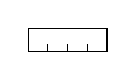
\begin{tikzpicture}
        \draw (0,0) rectangle (1,0.3);
        \foreach \i in {.25,.5,.75} {
          \draw (\i,0) -- (\i,.1);
        }
      \end{tikzpicture}
      Resulting range: $[0;2^{8\times 4}[=[0;2^{32}[\approx[0;4e^{10}]$
    \item \texttt{short} are stored on 2 cells
      \begin{tikzpicture}
        \draw (0,0) rectangle (.5,0.3);
        \foreach \i in {.25} {
          \draw (\i,0) -- (\i,.1);
        }
      \end{tikzpicture}
      ~Resulting range: $[0;2^{16}[=[0;65\,535]$
    \end{itemize}
  \end{block}

  \begin{block}{\alert{Problem}}
    \begin{itemize}
    \item \alert{Impossible to interpret a memory area without infos on data type stored}
    \item \structure{Remember:} C memory is a big magma (never forget!)
    \item Veeery different from Java where you have introspection abilities
    \end{itemize}
  \end{block}
\end{frame}
%%%%%%%%%%%%%%%%%%%%%%%%%%%%%%%%%%%%%%%%%%%%%%%%%%%%%%%%%%%%%%%%%%%%%%%%%%%
\section{Pointers}\toc
\subsection{Basics}
\begin{frame}{Pointers}
  \begin{block}{What is it?}
    \begin{itemize}
    \item \alert{Variable storing a memory address:} Pointer value = rank of a
      memory cell
    \item On 32 bits, I need 4 bytes to store an address since biggest
      address=$2^{32\times8}$\\  (8 bytes on 64 bits)
    \item Pointers are often written in hexadecimal (just a convention)
    \item Most of the time, numerical value is meaningless; where it points
      to is crucial

      \begin{center}
        \begin{tikzpicture}
          % Base line memory area
          \draw(0,0) -- (10.15,0) -- (10,.25) -- (10.15,.5) -- (10,.75) --
               (10.15,1) -- (0,1) -- (.15,.75) -- (0,.5) -- (.15,.25) -- (0,0);
          \foreach \i in { 1,2,4,5,6,7,8 } {
            \draw[loosely dotted](\i,0)     -- (\i,1);
            \draw[loosely dotted](\i+.25,0) -- (\i+.25,1);
            \draw[loosely dotted](\i+.5,0)  -- (\i+.5,1);
            \draw[loosely dotted](\i+.75,0) -- (\i+.75,1);
            \foreach \j in {0,1,2,3} {
              \node[right,rotate=270] at (\i+.13+\j*.25,1.05) 
                {\tiny 0x\pgfmathtruncatemacro{\res}{1024pt+(\i*4)+\j}%
                  \pgfmathdectoBase\mynumber{\res}{16}\mynumber};
            }
          }
          \foreach \i in {.25,.5,.75} {
            \draw(3+\i,1) -- (3+\i,.8);
          }
          \draw[loosely dotted](.5,0)   -- (.5,1); 
          \draw[loosely dotted](.75,0)  -- (.75,1); 
          \draw[loosely dotted](9,0)    -- (9,1); 
          \draw[loosely dotted](9.25,0) -- (9.25,1);
          \draw[loosely dotted](9.5,0)  -- (9.5,1);

          \node at (.3,.5) {\textbf{\ldots}};
          \node at (9.85,.5) {\textbf{\ldots}};

          % Example of a pointer in that memory
          \node at (3.5,1.2) {pointer p}; 
          \draw (3,0)    -- (3,1); 
          \draw (4,0)    -- (4,1); 

          \node at (3.5,.55) {0x414};
          \draw[*-stealth'] (3.5,0.3) .. controls (3.75,-0.5) and (4.8,-0.5) .. (5.12,0.1);          
        \end{tikzpicture}        
      \end{center}
    \end{itemize}
  \end{block}\vspace{-.7\baselineskip}

  \begin{block}<2->{But we can't interpret memory areas w/o info on stored type!}
    \begin{itemize}
    \item This information is given by the type of pointer
    \item[] \texttt{char* pc;}
      \begin{tikzpicture}[baseline]
        \draw (0,0) rectangle (1,0.4);
        \foreach \i in {.25,.5,.75} {
          \draw (\i,.3) -- (\i,.4);
        }

        \draw (1.75,0) rectangle (2,.4);
        \node at (1.87,0.2) {a};

        \draw[*-stealth'] (.5,0.3) .. controls (.5,-0.3) and (1.87,-0.3) .. (1.87,0);
      \end{tikzpicture}
      \hspace{2em}
      \texttt{int* pi;}
      \begin{tikzpicture}[baseline]
        \draw (0,0) rectangle (1,0.4);
        \foreach \i in {.25,.5,.75,  1.75,2,2.25} {
          \draw (\i,.3) -- (\i,.4);
        }

        \draw (1.5,0) rectangle (2.5,.4);
        \node at (2,0.2) {42};

        \draw[*-stealth'] (.5,0.3) .. controls (.5,-0.3) and (2,-0.3) .. (2,0);
      \end{tikzpicture}
    \item It is possible to store the address of a pointer of a pointer:
      \texttt{int ***p;}\\
      \structure{Remember:} types are to be read from right to left
    \end{itemize}
  \end{block}
\end{frame}
%%%%%%%%%%%%%%%%%%%%%%%%%%%%%%%%%%%%%%%%%%%%%%%%%%%%%%%%%%%%%%%%%%%%%%%%%%%%%%%%%%%%%%
\begin{frame}{Retrieving the address of something}
  \begin{block}{Motivation}
    \begin{itemize}
    \item Knowing that your pointer \texttt{p} points to 0x2342 is almost never relevant
    \item Knowing that it points to your variable \texttt{i} is what you need
    \end{itemize}
  \end{block}\vspace{-.5\baselineskip}
  \begin{block}{This is what the \alert{\&} operator does}
    \begin{itemize}
    \item \texttt{int i=42; \visible<2->{int *p=\alert{\&}i;}}
      \begin{tikzpicture}[baseline]
        \draw (0,0) rectangle (1,0.4);
        \foreach \i in {.25,.5,.75} {
          \draw (\i,.3) -- (\i,.4);
        }
        \node at (.5,0.2) {42};
        \node at (.5,.6) {i};

        \visible<2->{
          \draw (1,0) rectangle (2,.4);
          \foreach \i in {.25,.5,.75} {
            \draw (\i,.3) -- (\i,.4);
          }
          \draw[*-stealth'] (1.5,0.25) .. controls (1.5,-0.3) and (.5,-0.3) .. (.5,0);
          \node at (1.5,.55) {p};
        }        
      \end{tikzpicture}
      \visible<2->{\footnotesize(successive variables are (often) adjacent)}
    \end{itemize}
  \end{block}\vspace{-.5\baselineskip}

  \begin{block}<3->{We can now explain how scanf ``modifies its arguments''}
%    \medskip
    \begin{columns}
      \begin{column}{.2\linewidth}
\framebox{\tt\scriptsize\begin{minipage}{.5\linewidth}
\begin{tabbing}
int main() \{\\
~~int a;\\
~~scanf("\%d",\alert{\&}a);\\
\}
  \end{tabbing}    
  \end{minipage}}
      \end{column}
      \begin{column}{.2\linewidth}
      \begin{tikzpicture}
        % Stack container
        \draw[ultra thick] (0,2.5) -- (0,0) -- (2,0) -- (2, 2.5);
        \node at (1,-.3) {\bf Stack};
        
        % Stack frame of main 
        \draw (.2,.2) rectangle (1.8,.8);
        
        \node at (1.2,.5) [shape=rectangle,draw]  {?} ;
        \node at (.6,.45) {a};
                
        \node at (.55,1) {main};

        % Stack frame of scanf
        \draw (.2,1.2) rectangle (1.8,1.8);
          
        \node at (1.2,1.5) [shape=rectangle,draw]  {\phantom{?}} ;          
        \node at (.55,2) {scanf};

        \draw[*-stealth'] (1.15,1.5) .. controls (1.7,1.4) and (1.7,.5) .. (1.4,.5);

      \end{tikzpicture}
        
      \end{column}
      \begin{column}{.6\linewidth}
        \begin{itemize}
        \item \texttt{scanf} parameter: an address\\
          "\%d" tells how to interpret it
        \item That's copied over, but that's fine
        \item \texttt{scanf} can modify the \texttt{a} variable,\\
          even if it's not in its scope\\
          (\structure{remember:} C memory is a magma)
        \item other mystery: \visible<4->{variable amount of params\\
          \framebox{\texttt{man stdarg}} ;)}
        \end{itemize}
      \end{column}
    \end{columns}
  \end{block}
\end{frame}
%%%%%%%%%%%%%%%%%%%%%%%%%%%%%%%%%%%%%%%%%%%%%%%%%%%%%%%%%%%%%%%%%%%%%%%%%%%%%%%%%%%%%%%%%%%%
\newcommand{\strongstar}{\textbf{\textrm{*}}}
\begin{frame}{Fixing the triple() function}
  \begin{itemize}
  \item Remember our broken triple() function, which were unable to triple its argument
  \item That was because parameters are passed by value (copied over)
  \item To fix it, we simply use a pointer parameter
  \end{itemize}
    \begin{columns}
    \begin{column}{.35\linewidth}
      \framebox{\begin{minipage}{.3\linewidth}
          \tt\footnotesize  \begin{tabbing}
            \alert<3|handout:0>{void \textbf{triple}(int \strongstar a) \{}\\
            \alert<4|handout:0>{~~\strongstar a=(\strongstar a)*3;}\\
            \alert<5|handout:0>{~~return;}\\
            \}\\
            \\
            \alert<1|handout:0>{int \textbf{main}() \{}\\
            \alert<1|handout:0>{~~int x=12;}\\
            \alert<2|handout:0>{~~triple(\&x);}\\
            \alert<6|handout:0>{~~printf("x:~\%d",x);}\\
            \alert<7|handout:0>{~~return EXIT\_SUCCESS;}\\
            \}
          \end{tabbing}
        \end{minipage}}    
    \end{column}
    \begin{column}{.25\linewidth}
      \begin{tikzpicture}
        % Stack container
        \draw[ultra thick] (0,3.7) -- (0,0) -- (2,0) -- (2, 3.7);
        \node at (1,-.3) {\bf Stack};
        
        % Stack frame of main 
        \visible<1-6>{
          \draw (.2,.2) rectangle (1.8,.8);
          
          \node<-3|handout:0> at (1.2,.5) [shape=rectangle,draw]  {12} ;
          \node<4-> at (1.2,.5) [shape=rectangle,draw]  {36} ;
          \node at (.6,.45) {x};
                
          \node at (.55,1) {main};
        }

        \visible<3-4>{
          % Stack frame of max
          \draw (.2,1.2) rectangle (1.8,1.8);
          
          \node at (1.2,1.5) [shape=rectangle,draw]  {\phantom{36}} ;
          \node at (.6,1.45) {a};
          \draw[*-stealth'] (1.15,1.5) .. controls (1.8,1.4) and (1.8,.5) .. (1.5,.5);
          
          \node at (.55,2) {triple};
        }
      \end{tikzpicture}
    \end{column}
    \begin{column}{.3\linewidth}
      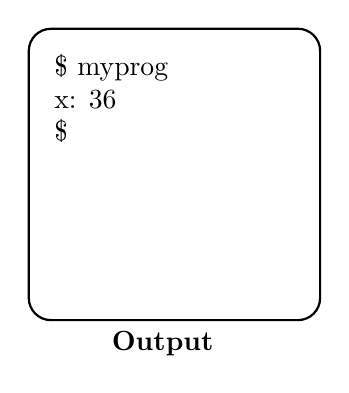
\begin{tikzpicture}
        \draw[thick,rounded corners=8pt] (0,0) rectangle (3.7,3.7);
        \node at (1.7,-.3) {\bf Output};

        \node[right] at (.2,3.2) {\$ myprog};
        \node<6->[right] at (.2,2.8) {x: 36};
        \node<7->[right] at (.2,2.4) {\$};

      \end{tikzpicture}
    \end{column}
  \end{columns}
  \begin{itemize}
  \item<7-> Pointers are powerful tools (that's why they are dangerous)
  \end{itemize}
\end{frame}
%%%%%%%%%%%%%%%%%%%%%%%%%%%%%%%%%%%%%%%%%%%%%%%%%%%%%%%%%%%%%%%%%%%%%%%%
\begin{frame}{Pointers Pitfalls}
  \Concept{There is reasons why students don't like pointers}
  \medskip

  \begin{block}{Pitfall \#1: * has a very heavy semantic}
    \begin{itemize}
    \item This little char is very loaded of semantic in C
    \item Forget only one * somewhere, and you're running into the segfault\\
      Same thing when writing a * too much
    \end{itemize}
  \end{block}\vspace{-.5\baselineskip}

  \begin{block}{Pitfall \#2: * actually has two differing meanings}
    \begin{itemize}
    \item \framebox{\texttt{int *p}} declares a \textbf{\alert{pointer
          variable}} \texttt{p} which is a pointer to an integer value
    \item \framebox{\texttt{*p}} is then the \textbf{\alert{pointed value}},
      interpreted according to the pointer type
    \item (that's actually three meanings when counting $\times$, the multiplication)
      \medskip
    \item \framebox{\texttt{int *p; p=12;}} selects where it points in memory
    \item \framebox{\texttt{int *p; *p=12;}} changes the memory in the pointed area
      \medskip

    \item Pascal was a bit more reasonable: \framebox{\texttt{INTEGER \^{}p}}
      vs. \framebox{\texttt{p\^{}}} {\small(at least other order)}
    \item In Java, there is no pointers, but reference to objects are close to
      that concept
    \end{itemize}
  \end{block}
\end{frame}
%%%%%%%%%%%%%%%%%%%%%%%%%%%%%%%%%%%%%%%%%%%%%%%%%%%%%%%%%%%%%%%%%%%%%%%%%%%%%%%%%%%
\begin{frame}{Pointer errors (and solutions)}
  \begin{block}{Most common error: errant mem access}
    \begin{itemize}
    \item Pointers make it easy to read or write anywhere in memory
    \item If the OS notices, program is sentenced an immediate death penalty
    \item When not, things get only worse\ldots
    \end{itemize}
  \end{block}
  \begin{block}{Memory errors are NASTY}
    \begin{itemize}
    \item Terse error message: "segmentation fault"
    \item Hard to correlate Effect and Fault
    \item To survive, you MUST know your tools: \underline{valgrind}
      and gdb (see practical)
    \end{itemize}
  \end{block}
  \begin{block}{Manipulating invalid pointers}
    \begin{itemize}
    \item The \texttt{NULL} value represents an invalid pointer. Often
      defined to 0
    \item Some pages at the beginning of the address space with no
      read/write perm
    \end{itemize}
  \end{block}
\end{frame}
%%%%%%%%%%%%%%%%%%%%%%%%%%%%%%%%%%%%%%%%%%%%%%%%%%%%%%%%%%%%%%%%%%%%%%%%%%%%%%%%%%%
\subsection{Pointers vs. Arrays}
\begin{frame}{Pointers vs. Arrays}
  \begin{block}{In C, \alert{Arrays are Pointers} (at least, most of the time)}
    \begin{itemize}
    \item Unfortunate heritage of C first years; One of the major pitfall for newcomers
    \item \framebox{\texttt{char array[8];}} (pointer to) a \textbf{reserved} area of 8
      bytes
      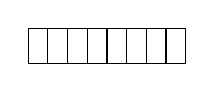
\begin{tikzpicture}[baseline]
        \draw (0,-0.1) rectangle (2,0.35);
        \foreach \i in {.25,.5,.75,1,1.25,1.5,1.75} {
          \draw (\i,0.35) -- (\i,-0.1);
        }
      \end{tikzpicture}
      \\
      As if it were an automatic \texttt{\alert{\&}array}: in pointer
      context, address of first cell
    \item \framebox{\texttt{int ai[~] = \{0,1,2\};}} (pointer to) a reserved+inited
       area of 3 ints
    \item \framebox{\texttt{char *str="blah"};} 2 areas: pointer + array
      \begin{tikzpicture}[baseline]
        \draw (0,-0.1) rectangle (.25,0.35);
        \draw (.75,-0.1) rectangle (2,0.35);
        \foreach \i in {1,1.25,1.5,1.75} {
          \draw (\i,0.35) -- (\i,-0.1);
        }
        \node [align=center] at (.875,.13) {\small b};
        \node [align=center] at (1.125,.13) {\small l};
        \node [align=center] at (1.375,.10) {\small a};
        \node [align=center] at (1.625,.13) {\small h};
        \node [align=center] at (1.875,.10) {\scriptsize$\backslash\!\emptyset$};

        \draw[*-stealth'] (.1,.13) .. controls (.35,-0.3) and (.6,-0.3).. (.87,-.1);
      \end{tikzpicture}

    \medskip
    \item \framebox{\texttt{void max(int ai[~])}} $\approx$
      \framebox{\texttt{void max(int *ai)}}  Expects an int pointer \\[2pt]
      Explains why strings don't take any \& in scanf: they already
      are pointers
    \item \framebox{\texttt{void max(int ai[32])}} Similar, but whole array is
      copied on stack
    \end{itemize}
  \end{block}

  \begin{block}{Considering Pointers as Arrays}
    \begin{itemize}
    \item \framebox{\texttt{int *pi=}\ldots\texttt{; pi[3];}} This is valid;
      Behave as expected\\
      {\small (no bound checking, as usual in C)}
    \end{itemize}
  \end{block}

\end{frame}
%%%%%%%%%%%%%%%%%%%%%%%%%%%%%%%%%%%%%%%%%%%%%%%%%%%%%%%%%%%%%%%%%%%%%%%%%%%%%%%%%%%
\begin{frame}{Pointer Arithmetic}
  \begin{block}{Adding and subtracting integers to pointers is valid} 
    \begin{itemize}
    \item It represents a \textbf{\alert{shift in cell (not in bytes)}}
    \end{itemize}
  \end{block}
  \begin{columns}
    \begin{column}{.25\linewidth}
      \framebox{\begin{minipage}{.3\linewidth}
          \tt\footnotesize  \begin{tabbing}
            int *pi=0x400;\\
            pi=pi+3;\\
            printf("pi:\%x$\backslash$n",pi);
          \end{tabbing}
        \end{minipage}}    
    \end{column}
    \begin{column}{.55\linewidth}
      \begin{tikzpicture}[baseline]
        % Base line memory area
        \draw(.75,0) -- (8,0);
        \draw(.75,1) -- (8,1);
        \draw[decorate,decoration={zigzag,amplitude=2pt}] (.75,0) -- (.75,1);
        \draw[decorate,decoration={zigzag,amplitude=2pt}] (8,0) -- (8,1);

          \foreach \i in { 2,3,4,5,6,7 } {
            \draw[loosely dotted](\i,0)     -- (\i,1);
            \draw[loosely dotted](\i+.25,0) -- (\i+.25,1);
            \draw[loosely dotted](\i+.5,0)  -- (\i+.5,1);
            \draw[loosely dotted](\i+.75,0) -- (\i+.75,1);
            \foreach \j in {0,1,2,3} {
              \node[right,rotate=270] at (\i+.13+\j*.25,1.05) 
                {\tiny 0x\pgfmathtruncatemacro{\res}{1016pt+(\i*4)+\j}%
                  \pgfmathdectoBase\mynumber{\res}{16}\mynumber};
            }
          }
          \foreach \i in {.25,.5,.75} {
            \draw(1+\i,1) -- (1+\i,.8);
          }

          % Example of a pointer in that memory
          \node at (1.5,1.2) {pointer p}; 
          \draw (1,0)    -- (1,1); 
          \draw (2,0)    -- (2,1); 

          \draw[*-stealth'] (1.5,0.5) .. controls (1.75,-0.5) and (2,-0.5).. (2.12,0.1)
            node[midway,below] {before};          
          \draw[*-stealth'] (1.5,0.5) .. controls (2.75,-0.5) and (5,-0.5).. (5.12,0.1)
            node[midway,below] {after};          
      \end{tikzpicture}
    \end{column}    
  \end{columns}
  \begin{itemize}
  \item Value change in *pi:  \texttt{value\_after}= \texttt{value\_before}+\texttt{sizeof(int)}$\times3$\\
    because it points on integers
  \end{itemize}
  \begin{block}{Subtracting 2 pointers is valid} 
    \begin{itemize}
    \item It gives the shift between them (in cells, not in byte)
    \end{itemize}
  \end{block}

  \concept{Other arithmetic operations are \textbf{not valid} on pointers}

  \begin{block}{Pointers, Arithmetic, and Arrays}
    \begin{itemize}
    \item \framebox{\texttt{p[i]}} is equivalent to \framebox{\texttt{*(p+i)}}
      ~~~(that is why we count elements from 0)
    \end{itemize}
  \end{block}
\end{frame}
%%%%%%%%%%%%%%%%%%%%%%%%%%%%%%%%%%%%%%%%%%%%%%%%%%%%%%%%%%%%%%%%%%%%%%%%%%%%%%%%%%%
\subsection{Casting Pointers}\subtoc
\begin{frame}{Casting Data}
  \vspace{-.5\baselineskip}
  \begin{block}{What is it?}
    \begin{itemize}\vspace{-.2\baselineskip}
    \item This is the well known \framebox{\texttt{int a =}
        \textbf{(int)}\texttt{b}} notation. More generally, \framebox{\texttt{(type)}}
    \item It is used to convert something in a type into something else
    \item Two meanings, depending on whether it's applied on scalars or
      pointers
    \item Quite the same story in Java/C++, actually
    \end{itemize}
  \end{block}\vspace{-.5\baselineskip}

  \begin{block}{Casting Scalars: Converting values}
    \begin{itemize}\vspace{-.2\baselineskip}
    \item \texttt{double d = 5.7;} ~~~~
      \visible<2->{
        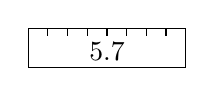
\begin{tikzpicture}[baseline]
          \draw (0,0) rectangle (2,0.5);
          \foreach \i in {.25,.5,.75,1,1.25,1.5,1.75} {
            \draw (\i,0.5) -- (\i,.4);
          }
          \node at (1,.2) {5.7};
      \end{tikzpicture}}

      \texttt{int i = (int)d;} ~~~~
      \visible<2->{
        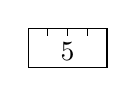
\begin{tikzpicture}[baseline]
          \draw (0,0) rectangle (1,0.5);
          \foreach \i in {.25,.5,.75} {
            \draw (\i,0.5) -- (\i,.4);
          }
          \node at (.5,.2) {5};
      \end{tikzpicture}}

    \item<2-> Casting Scalars can lead to:
      \begin{itemize}
      \item Change the memory representation of the value
      \item Change the amount of memory needed to represent the value
      \item Lead to precision loss (!)
      \end{itemize}
    \end{itemize}
  \end{block}\vspace{-.5\baselineskip}

  \begin{block}<3->{Casting Pointers: Changing the semantic}
    \begin{itemize}\vspace{-.2\baselineskip}
    \item It's written exactly the same way \ldots\ but the meaning is very different
    \item Let's look again at the Java/C++ semantic of reference casting
    \end{itemize}
  \end{block}
\end{frame}
%%%%%%%%%%%%%%%%%%%%%%%%%%%%%%%%%%%%%%%%%%%%%%%%%%%%%%%%%%%%%%%%%%%%%%%%
\begin{frame}{Casting Objects in Java/C++}
  \begin{block}{Java/C++ Semantic Casting}
    \begin{columns}
      \begin{column}{.3\linewidth}
        \framebox{\begin{minipage}{.3\linewidth}
            \tt\footnotesize  
            \begin{tabbing}
Toto to = new Tutu();\\
Tutu tu = (Tutu)to;
            \end{tabbing}      
          \end{minipage}}
      \end{column}

      \begin{column}{.3\linewidth}
        \begin{tikzpicture}[decoration={random steps,amplitude=1pt,segment length=3pt}]%[show background grid]
          % Object
          \draw (2,-.5) rectangle (3,1);
          \node at (2.5,.8) {\small\tt Tutu};
          \draw (2,.65) -- (3,.65);
          \foreach \y in {.53,.4,.31,.2,  .05,-.1,-.2,-.32} {
            \draw[decorate] (2.2,\y) -- (2.8,\y);
          }
          \draw (2,.15) -- (3,.15);
          
          % Variables
          \node at (0 ,.1) {tu};
          \node[shape=rectangle,draw] at (.5,.1) {\phantom{to}};
          
          \node at (0 ,.7) {to};
          \node[shape=rectangle,draw] at (.5,.7) {\phantom{to}};
          
          % References
          \draw[*-stealth'] (0.45,.1) -- (2,.65)
             node[sloped,midway,below] {\tiny as a Tutu};
          \draw[*-stealth'] (0.45,.7) -- (2,.8) 
             node[sloped,midway,above] {\tiny as a Toto};
        \end{tikzpicture}
      \end{column}
    \end{columns}
    
    \begin{itemize}
    \item Through \texttt{tu}, I consider the object to be a \texttt{Tutu}
    \item It does not change the value of the object, only what I expect from it
    \item Only valid if \texttt{Tutu extends Toto} (and useless if \texttt{Toto extends Tutu})
    \end{itemize}    
  \end{block}
  \begin{block}{Side note: Static vs. Dynamic typing is a creepy part of Java}
    \begin{itemize}
    \item Casts relax constraints at compilation time; Enforced at execution time\\
      That is what \texttt{TypeCastException} is made for
    \item Guessing which method gets called is sometimes excessively
      difficult\\
      {\small Check again TD4 of POO if you forgot}
    \item But it's hard to depreciate the Java typing system in a course on C\ldots
    \end{itemize}
  \end{block}
\end{frame}
\end{Coupe}
%%%%%%%%%%%%%%%%%%%%%%%%%%%%%%%%%%%%%%%%%%%%%%%%%%%%%%%%%%%%%%%%%%%%%%%%%%%%%%%%%%%%%%
\begin{frame}{Casting Pointers in C}
  \begin{block}{They change the Pointer Semantic}
    \begin{itemize}
    \item The numeric value of the pointer does not change
    \item But the dereferencing it completely different
    \item Also has a huge impact on pointer arithmetic
    \end{itemize}
  \end{block}

  \begin{columns}
    \begin{column}{.25\linewidth}
      \framebox{\begin{minipage}{.3\linewidth}
          \tt\footnotesize  \begin{tabbing}
            int a;\\
            int *pi=\&a;\\
            char *pc=pi;\\
            pi++;\\
            pc++;
          \end{tabbing}
        \end{minipage}}    
    \end{column}
    \begin{column}{.55\linewidth}
      \begin{tikzpicture}[baseline]
        \foreach \cell in {1,2,3} {
          \foreach \i in {.25,.5,.75} {
            \draw[loosely dotted] (\cell+\i,0) -- (\cell+\i,1);
            \draw (\cell,0) rectangle (\cell+1,1); 
          }
        }
        
        \node at (1.5,.5) {a}; 
        \node at (2.5,.5) {pi}; 
        \node at (3.5,.5) {pc}; 


        \draw[*-stealth'] (2.5,0.2) .. controls (2.25,-0.5) and (1.25,-0.5).. (1.12,0.1);
        \draw[*-stealth'] (3.5,0.2) .. controls (3.25,-0.5) and
        (1.25,-0.5).. (1.12,0.1);
        \visible<2->{
          \node at (2.5,-.5) {before};

          \draw[*-stealth'] (2.5,0.8) .. controls (2.25,1.2) and (2.25,1.2).. (2.12,1);
          \draw[*-stealth'] (3.5,0.8) .. controls (3.25,1.1) and (1.5,1.1).. (1.37,1);
          \node at (2.5,1.3) {after};
        }

      \end{tikzpicture}
    \end{column}    
  \end{columns}

  \bigskip\bigskip
  \concept{Types in C: no formal semantic, only denote size in memory}
\end{frame}
%%%%%%%%%%%%%%%%%%%%%%%%%%%%%%%%%%%%%%%%%%%%%%%%%%%%%%%%%%%%%%%%%%%%%%%%%%%
\begin{frame}{Generic Pointers}
  \begin{block}{Generic pointers are sometimes handy}
    \begin{itemize}
    \item To describe pointers that can point to differing data\\
      \structure{Example:} in scanf, how to interpret the pointer is given by
      the format
    \item To describe pointers to \textit{raw} data (ie, you don't care about
      the pointed type)\\
      \structure{Example:} When copying memory chunk over, content does not matter
    \end{itemize}
  \end{block}
  \begin{block}{That is what void* is made for}
    \begin{itemize}
    \item Modern compiler even allow you to do pointer arithmetic on them
    \item[] supposing that \texttt{sizeof(void)=1}, which is \ldots\ arbitrary
    \item Older compiler force you to cast them to \texttt{char*} before
    \end{itemize}
  \end{block}
\end{frame}
%%%%%%%%%%%%%%%%%%%%%%%%%%%%%%%%%%%%%%%%%%%%%%%%%%%%%%%%%%%%%%%%%%%%%%%%%%%
\section{Dynamic Memory}\subtoc
\subsection{Memory Blocs and Pointers}
\begin{frame}{Dynamic Memory}
  \vspace{-.6\baselineskip}
  \begin{block}{Motivation}
    \begin{itemize}
    \item Arrays are statically sized in C (\textit{i.e.} their size must be
      known at compilation)
    \item It is forbidden to write:
      \framebox{\begin{minipage}{.3\linewidth}
          \tt\footnotesize  \begin{tabbing}
            int n;\\
            scanf("\%d",\&n);\\
            int tab[n];
          \end{tabbing}
        \end{minipage}}    
      because \texttt{n} is only known at execution
    \item (this is not true in C99, but C99 not widely spread yet)
    \end{itemize}
  \end{block}\vspace{-.6\baselineskip}

  \begin{block}{Solution}
    \begin{itemize}
    \item Directly request memory chunks from the system
    \item Manage them yourself
    \item And return them to the system when you're done
    \end{itemize}
  \end{block}\vspace{-.6\baselineskip}

  \begin{block}{Remember the Memory Layout of a Process}
    \begin{center}
    \begin{tikzpicture}
      \draw (0,0) -- (6,0) -- (6,1) -- (0,1) -- (0,0);
      \draw (7.8,0) -- (10.3,0) -- (10.3,1) -- (7.8,1) -- (7.8,0);
      \draw (3,0) -- (3,1);
      \node at (1.5,0.73) {\textbf{Data}};
      \node at (1.5,0.25) {Code+Globals};

      \node at (4.5,0.73) {\textbf{Heap}};
      \node at (4.5,0.25) {Dynamic Memory};

      \node at (9,0.73) {\textbf{Stack}};
      \node at (9,0.25) {Stack Frames};
      \draw[-stealth',thick] (6,.5) -- (6.5,.5);
      \draw[-stealth',thick] (7.8,.5) -- (7.3,.5);
      
      \node at (6.9,.5) {$\emptyset$};
      \node at (0,-.2) {0};
      \node at (10.3,-.2) {4Gb};
    \end{tikzpicture}
    \end{center}\vspace{-1.5\baselineskip}
    \begin{itemize}
    \item The idea is to request memory from the heap
    \end{itemize}
  \end{block}
\end{frame}
%%%%%%%%%%%%%%%%%%%%%%%%%%%%%%%%%%%%%%%%%%%%%%%%%%%%%%%%%%%%%%%%%%%%%%%%
\begin{frame}{Requesting Memory Chunks from the heap}
  \begin{block}{The several ways of doing so}
    \begin{itemize}
    \item As usual, there is a high level and a low level API
    \item At low-level, the \texttt{brk()} syscall allows to move the heap
      boundary\\
      And you are on your own to manage its content (emacs does it)
    \end{itemize}
  \end{block}
  \begin{block}{malloc() and friends}
    \begin{itemize}
    \item This higher level API directly gives memory chunks in heap\\
      {and deal automatically with \texttt{brk()}}
    \item There is only 3 functions to know

      \smallskip
      \begin{tabular}{rl}
      \texttt{\#include <stdlib.h>}\\
      \texttt{void*malloc(int size)}& Request a new memory chunk\\
      \texttt{void free(void*p)}& Return a memory chunk\\
      \texttt{void*realloc(void*p,int size)}& Expend a memory chunk        
      \end{tabular}
    \end{itemize}
  \end{block}
\end{frame}
%%%%%%%%%%%%%%%%%%%%%%%%%%%%%%%%%%%%%%%%%%%%%%%%%%%%%%%%%%%%%%%%%%%%%%%%
\begin{frame}{Understanding malloc and friends}
  \begin{block}{Function Semantic}
    \begin{itemize}
    \item malloc() requests a new memory chunk and return the address of beginning\\
      If there is not enough free memory, it returns NULL
    \end{itemize}
  \end{block}\vspace{-.5\baselineskip}
  \begin{block}{Think of a land registry for the memory}
    \begin{itemize}
    \item \texttt{void *A=malloc(12);}
      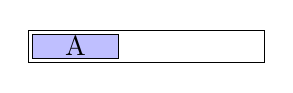
\begin{tikzpicture}[baseline]
        \draw (0,-.1) rectangle (3,.3);
        \draw[fill=blue!25] (.05,-.05) rectangle (1.15,.25) node[midway] {A};
      \end{tikzpicture}
    \item \texttt{void *B=malloc(5);~}
      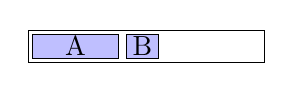
\begin{tikzpicture}[baseline]
        \draw (0,-.1) rectangle (3,.3);
        \draw[fill=blue!25] (.05,-.05)  rectangle (1.15,.25) node[midway] {A};
        \draw[fill=blue!25] (1.25,-.05) rectangle (1.65,.25) node[midway] {B};
      \end{tikzpicture}
    \item \texttt{free(A);~~~~~~~~~~~}
      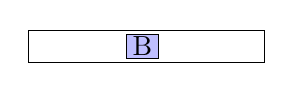
\begin{tikzpicture}[baseline]
        \draw (0,-.1) rectangle (3,.3);
        \draw[fill=blue!25] (1.25,-.05) rectangle (1.65,.25) node[midway] {B};
      \end{tikzpicture}
    \item \texttt{void *C=malloc(6);~}
      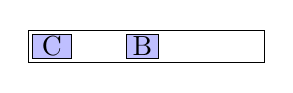
\begin{tikzpicture}[baseline]
        \draw (0,-.1) rectangle (3,.3);
        \draw[fill=blue!25] (1.25,-.05) rectangle (1.65,.25) node[midway] {B};
        \draw[fill=blue!25] (.05,-.05) rectangle (.55,.25) node[midway] {C};
      \end{tikzpicture}
    \item \texttt{C=realloc(C,13);~~~}
      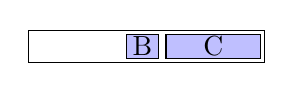
\begin{tikzpicture}[baseline]
        \draw (0,-.1) rectangle (3,.3);
        \draw[fill=blue!25] (1.25,-.05) rectangle (1.65,.25) node[midway] {B};
        \draw[fill=blue!25] (1.75,-.05) rectangle (2.95,.25) node[midway] {C};
      \end{tikzpicture}
    \end{itemize}
  \end{block}\vspace{-\baselineskip}

  \begin{block}{As usual in C}
    \begin{itemize}
    \item There is no protection mechanism here: Mess it up and you'll get a segfault
    \item Two surviving strategies:
      \begin{itemize}
      \item Avoid issues through best practices
      \item Solve issues through debugging tools
      \end{itemize}
    \end{itemize}
  \end{block}
\end{frame}
%%%%%%%%%%%%%%%%%%%%%%%%%%%%%%%%%%%%%%%%%%%%%%%%%%%%%%%%%%%%%%%%%%%%%%%%%%%%%%%%%%%
\begin{frame}{Best Practices about Dynamic Memory}
  \begin{block}{\alert{Rule \#1:} Only access to reserved areas}
    \begin{itemize}
    \item \structure{Land Registry Analogy:} Only build stuff on land that you own
    \end{itemize}
    \begin{columns}
      \begin{column}{.4\linewidth}
        \begin{center}
          \framebox{\begin{minipage}{.3\linewidth}
          \tt\footnotesize  \begin{tabbing}
            int *A;\\
            *A=1;\\
            A=malloc(sizeof(int));
          \end{tabbing}
        \end{minipage}}            

      \medskip
      \alert{Error! A used before malloc!}

      \medskip
      {\small (buy it before building)}
    \end{center}
  \end{column}
  \begin{column}{.4\linewidth}
    \begin{center}
      \framebox{\begin{minipage}{.3\linewidth}
          \tt\footnotesize  \begin{tabbing}
            int *A=malloc(sizeof(int));\\
            free(1);\\
            *A=1;
          \end{tabbing}
        \end{minipage}}            

      \medskip
      \alert{Error! A used after free!}

      \medskip
      {\small(forget it after selling it)}
    \end{center}
  \end{column}
\end{columns}\medskip
\begin{itemize}
\item You'll have similar symptoms in both case
  \begin{itemize}
  \item If you are lucky, segfault (error signaled where the fault is)
  \item If not, some memory pollution (probably a later segfault, harder to
    diagnose)
  \end{itemize}

\end{itemize}

  \end{block}
\end{frame}
%%%%%%%%%%%%%%%%%%%%%%%%%%%%%%%%%%%%%%%%%%%%%%%%%%%%%%%%%%%%%%%%%%%%%%%%%%%%%%%%%%%
\begin{frame}{Best Practices about Dynamic Memory}
  \begin{block}{\alert{Rule \#2:} To any malloc(), one and only one free()}
    \begin{itemize}
%    \item \structure{Land Registry Analogy:} Sell everything back (once)

    \item If you forget the \texttt{free()}, there is a \textbf{\alert{memory leak}}
      \begin{itemize}
      \item The system assumes that this area is used where it's not anymore
      \item Ok to have a few memleaks. Too much of them will exhaust system resources
      \item Slows down (swap); malloc() eventually returns
        NULL (or OOM killer)
      \end{itemize}

    \item If you call \texttt{free()} twice (\textbf{\alert{double free}}), strange things will occur

      \begin{columns}
        \begin{column}{.26\linewidth}
          \begin{center}
            \framebox{\begin{minipage}{.25\linewidth}
                \tt\footnotesize  \begin{tabbing}
                  int *A=malloc(12);\\
                  free(A);\\
                  int *\alert{B}=malloc(12);\\
                  free(A);
                \end{tabbing}
              \end{minipage}}            
          \end{center}
        \end{column}
        \begin{column}{.7\linewidth}
          $\leadsto$ Probably frees B \ldots\\
          Unfriendly if A and B are in two separate modules
        \end{column}
      \end{columns}

      \begin{itemize}
      \item That is why modern malloc implementations try to detect this situation
      \item And kill faulty program as soon as the error is detected
      \end{itemize}
    \end{itemize}


  \end{block}
\end{frame}
